\documentclass{VUMIFPSbakalaurinis}
\usepackage{float}
\usepackage{hyperref}
\usepackage{algorithmicx}
\usepackage{algorithm}
\usepackage{algpseudocode}
\usepackage{amsfonts}
\usepackage{amsmath}
\usepackage{bm}
\usepackage{caption}
\usepackage{color}
\usepackage{graphicx}
\usepackage{listings}
\usepackage{subcaption}
\usepackage{wrapfig}
\usepackage{biblatex}
\usepackage{microtype}
\usepackage{mathtools}
\usepackage{multirow}
\usepackage{graphics}


% Titulinio aprašas
\university{Vilniaus universitetss}
\faculty{Matematikos ir informatikos fakultetas}
\institute{Informatikos institutas}  % Užkomentavus šią eilutę - institutas neįtraukiamas į titulinį
\department{Programų sistemų bakalauro studijų programa}
\papertype{Laboratorinio darbo ataskaita}
\title{Vaizdų klasifikavimas naudojant konvoliucinius neuroninius tinklus}
\titleineng{Image Classification Using CNN}
\author{Armintas Pakenis}
% \secondauthor{Vardonis Pavardonis}   % Pridėti antrą autorių
\supervisor{prof. dr. Olga Kurasova}
\reviewer{prof. dr. Olga Kurasova}
% \addsignatureplaces{} % prideda parašų vietas tituliniame puslapyje
\date{Vilnius – \the\year}

\bibliography{bibliografija}

\begin{document}
\maketitle

%% Padėkų skyrius
% \sectionnonumnocontent{}
% \vspace{7cm}
% \begin{center}
%     Padėkos asmenims ir/ar organizacijoms
% \end{center}

\tableofcontents

\section{Užduoties tikslas}
Užduoties tikslas — išbandyti sukurti skirtingas konvoliucinio neuroninio 
tinklo architektūras ir rasti iš išbandytų geriausią. Rašytas programos
kodas naudoja PyTorch biblioteką.
Naudotos programos kodą 
galima rasti GitHub repositorijoje: 
\href{https://github.com/ArmintasP/Computational-intelligence/tree/main/Lab4}{\color{cyan}{https://github.com/ArmintasP/Computational-intelligence/tree/main/Lab4}}.

\subsection{Duomenys}
Naudotas CIFAR-10 duomenų rinkinys
\href{https://www.cs.toronto.edu/~kriz/cifar.html}{\color{cyan}{https://www.cs.toronto.edu/~kriz/cifar.html}}.

Rašyta programa buvo išskaidyta į dvi dalis: viena apdoruoja duomenis,
kita treniruoja modelį. Programos dalys skirtingose Jupyter
užrašų knygutėse.

CIFAR-10 duomenų rinkinys buvo užkoduotas failuose. Failai buvo
nuskaitomi panaudojant metodą "unpickle" iš to paties 
duomenų rinkinio autorių puslapo. Likusi pirmos programos dalies
kodo dalis originali, kur atrenkamos RGB reikšmės ir atkuriamos nuotraukos .jpg formatu.
Kiekvienos klasės nuotraukos išsaugomos atskirame kataloge su tos
klasės pavadinimu.

Vaizdų klasių 10: lėktuvai, automobiliai, paukščiai,
katės, elniai, šunys, varlės, arkliai, laivai ir sunkvežimiai.

Originalus CIFAR-10 rinkinys pateikia 6000 nuotraukų kiekvienai klasei.
Iš viso 10 klasių, 50000 nuotraukų skirtų mokymui ir 10000 testavimui.
Po failų apdorojimo, 50000 ir 10000 nuotraukų buvo sumaišytos ir
padalintos atsitiktinai pagal santykiu 7:3. Nuotraukų dydis: $32 \times 32$.

\subsection{Įranga}
Modelio treniravimas vyko ant asmeninio kompiuterio su
AMD Ryzen 5 5600G APU (CPU) ir 32 GB RAM.

\section{Modelių architektūros}

Nagrinėtos 3 architektūros: A, B ir C (žr. \ref{img:arch-list} pav.).
A architektūra paremta LeNet modelio architektūra, atlikti
tokie pakeitimai: įvesties nuotraukos ilgis ir plotis padidinti
iki 32 pikselių, prieš priešpaskutinį sluoksnį atsiranda 
išmetimo (Dropout) sluoksnis. Lyginant architektūras, užfiksuoti šie hiperparametrai:
\begin{itemize}
  \item Aktyvacijos funkcija — ELU.
  \item Paketo dydis —  32.
  \item Išmetimo sluoksnio tikimybė —  0.4.
  \item Optimizavimo algoritmas — Adam.
  \item Nuostolių funkcija — kryžminė entropija.
  \item Mokymosi greitis — 0,001.
  \item Epochų skaičius - 30.
\end{itemize} 

\noindent Duomenų rinkinio mokymo duomenims buvo naudotos šios
augmentacijos:
\begin{itemize}
  \item Spalvų variacija (color jitter).
  \item Atsitiktinis horizontalus apvertimas.
  \item Atsitiktinis RGB nuotraukos pavertimas į monochromatinę.
\end{itemize}

\begin{figure}[H]
  \centering
  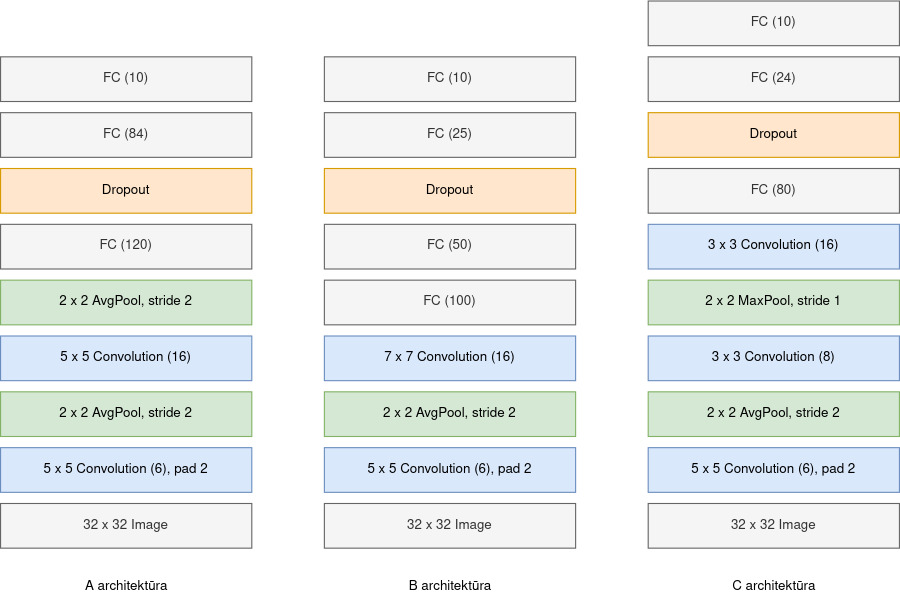
\includegraphics[scale=0.5]{img/arch-list.jpg}
  \caption{Trys architektūros. Sluoksniai ar jų operacijos
  taikomi iš apačios į viršų}
  \label{img:arch-list}
\end{figure}


\subsection{Architektūrų palyginimas}

A modelis turi 83 126 parametrų, B — 171 861, C — 159 218.

Iš mokymo rezultatų matyti, kad tikslumas ir skirtumas tarp
mokymo bei validavimo tikslumo nesiskiaria architektūrose
A ir C (žr. \ref{img:a-results} ir \ref{img:c-results} pav.).
Nors C turi bene dvigubai daugiau parametrų nei A, C modelis
nepronoko A. Blogiausiai pasirodė B modelis (žr. ref{img:b-results} pav.) 
su daugiausiai parametrų. Pašalinus sujungimo sluoksnį (AvgPool) ir
panaudojus pilnai sujungtą, rezultatai net pablogėjo: nuo 20 epochos
validavimo tikslumas nedidėjo, kai didėjo treniravimo — ženklas,
kad B modelis persimokė.

Galima daryti išvadą, kad šitame klasifikavimo uždaviny su
esamu rinkiniu daug svarbiau turėti konvoliucinius sluoksnius. 
Tačiau kaip matoma iš C pavyzdžio, sluoksniai papildomo  tikslumo
ženkliai nepradėjo. Nors C pirmosios epochos turėjo
geresnius tikslumus, griežtai to patvirtinti negalima, kadangi
tai galėjo būti sutapimas dėl atsitiktinai inicializuotų
svorių mokymo pradžioje.


\begin{figure}[H]
  \centering
  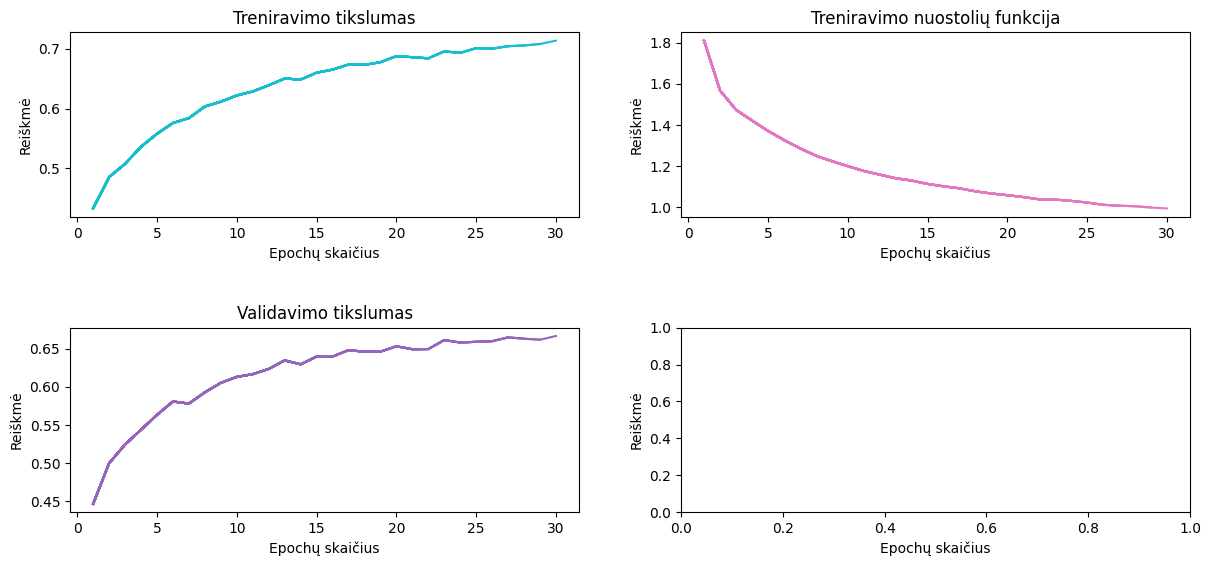
\includegraphics[scale=0.5]{img/A.png}
  \caption{A architektūros tikslumo ir nuostolių funkcijos grafikai}
  \label{img:a-results}
\end{figure}

\begin{figure}[H]
  \centering
  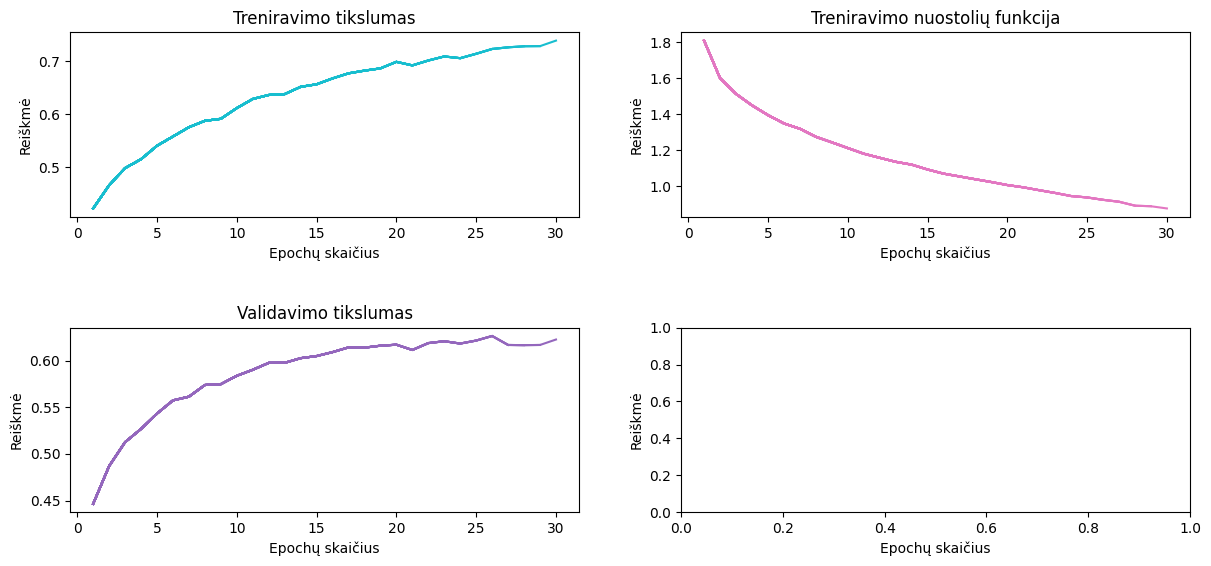
\includegraphics[scale=0.5]{img/B.png}
  \caption{A architektūros tikslumo ir nuostolių funkcijos grafikai}
  \label{img:b-results}
\end{figure}


\begin{figure}[H]
  \centering
  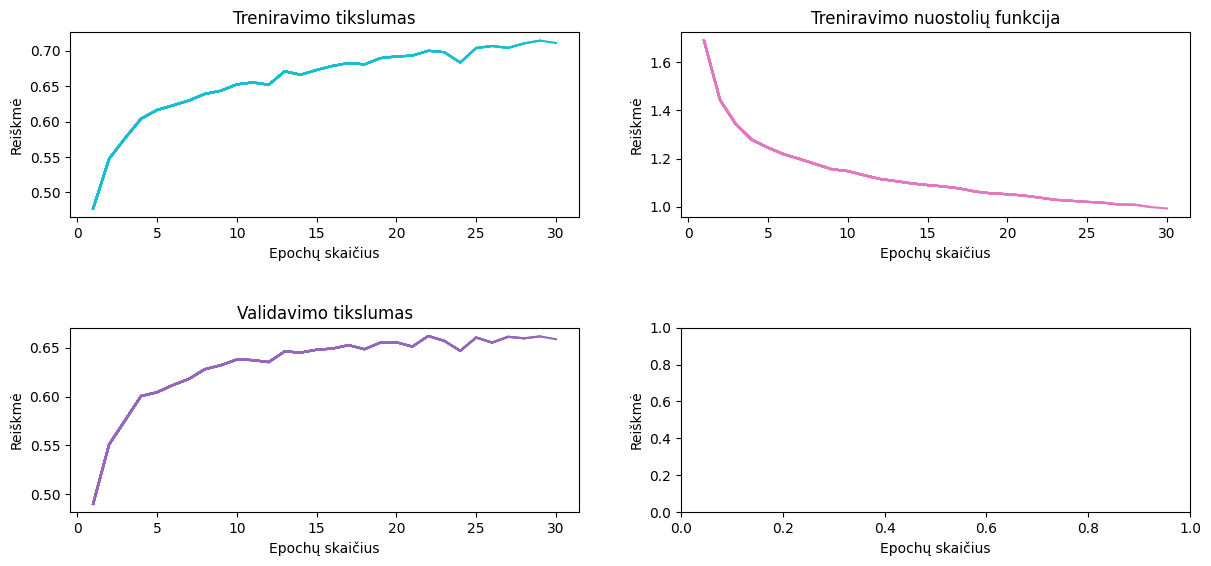
\includegraphics[scale=0.5]{img/C.png}
  \caption{A architektūros tikslumo ir nuostolių funkcijos grafikai}
  \label{img:c-results}
\end{figure}


\section{Hiperparametrų įtaka konvoliuciniam neuroniniam tinklui}

Toliau nagrinėjama tik A modelio architektūra su skirtingais 
specifiniais hiperparametrais.

Epochų skaičius, mokymosi greitis, paketo dydis ir skirtingų
augmentacijų poveikis mokymosi ir validavimo tikslumui nebus nagrinėjami.
Šie hiperparametrai nekis ir bus atitinkamai 10, 0,001, 32 ir 
anksčiau minėtos augmentacijos. Nuostolių funkcija irgi išliks
kryžminė entropija.

Rezultatuose (žr. \ref{tab:hiperparametrai} lentelę) matoma, kad
stohastinio gradiento nusileidimo optimizavimo algoritmas veikia
blogiau nei Adam algoritmas. Tačiau taip yra todėl, kad SGD yra
taikomas paketui, kurio dydis yra lygus vienetui. Lentelėje pateikti
hiperparametrai buvo keisti paliekant tą patį paketo dydį. Tačiau atlikus
papildomą modelio apmokymą su 2 eilutės duomenimis (naudojant SGD optimizatorių)
ir pakeitę paketo dydį į 1, gauta nuostolių funkcijos reikšmė yra arti 1,23, o
mokymosi tikslumas su validavimo — 59,05 ir 60,03 \%. Tad parinkus tinkamą
paketo dydį, SGD algoritmas veikia beveik tiek pat gerai, kiek Adam. 
Tačiau atlikus šį papildomą apmokymą su vieneto dydžio paketais 
modelio apmokymas užtruko dvigubai ilgiau (18 minučių).

Trečioje lentelės eilutėje matome geriausias pasiektas statistikas,
kur išmetimo sluoksnio tikimybė yra 0; kitaip tariant, kai jo nėra. 
Tačiau verta atkreipti dėmesį, kad išmetimo sluoksnis yra taikomas
modelio permokymo problemai spręsti. Šiuo atveju tarp mokymosi tikslumo
ir validavimo tikslumo yra $66,17 \% - 61,94 \% = 4,23 \%$. Lyginant su kitomis
eilutėmis panašu, kad su tokiu išmetimo sluoksnio hiperparametru mūsų modelis
persimokys. Ketvirtoje eilutėje matome aukštą išmetimo sluoksnio tikimybę,
tačiau ji per daug aukšta ir geriausiai, panašu, kad robastiškumui pasiekti
geresnė tikimybė yra $0,4$, ypač jei norima, kad modelis nepersimokytų.

Paskutiniose trijose eilutėse išbandomos skirtingos funkcijos. Blogiausiai
tam tinka sigmoidinė. Nors modelsi nėra architektūriškai didelis,
panašu, kad artėjama prie nykstančių gradientų ir nuo to kenčia
mokymosi tikslumas. Panašu, kad geriausi rezultatai gali būti pasiekiami
naudojant ReLU funkciją, kuri, priešingai nei ELU, negali įgyti neigiamų reikšmių.
Būtent išmokytą modelį, kuris naudoja ReLU funkciją ir kitus tos lentelės eilutės
hiperparemtrus, laikysime geriausiu, kadangi jis pasiekė aukščiausią validavimo
tikslumą, skirtumas tarp mokymosi tikslumo ir validavimo tikslumo mažesnis nei 
3 eilutės, o nuostolių funkcijos reikšmė irgi nėra reikšmingai nutolusi nuo 3
eilutės reikšmės (1,03).


% Please add the following required packages to your document preamble:
% \usepackage[table,xcdraw]{xcolor}
% If you use beamer only pass "xcolor=table" option, i.e. \documentclass[xcolor=table]{beamer}
\begin{table}[]
  \centering
  \caption{Tikslumo ir nuostolių funkcijos priklausomybė nuo hiperparametrų}{
    \begin{tabular}{|c|c|c|c|c|c|}
      \hline
      \textbf{\begin{tabular}[c]{@{}c@{}}Optimizavimo \\ algoritmas\end{tabular}} & \textbf{\begin{tabular}[c]{@{}c@{}}Išmetimo\\  sluoksnio tik.\end{tabular}} & \textbf{\begin{tabular}[c]{@{}c@{}}Aktyvacijos\\  f-ija\end{tabular}} & \textbf{\begin{tabular}[c]{@{}c@{}}Nuostolių\\  f-ijos reikšmė\end{tabular}} & \textbf{\begin{tabular}[c]{@{}c@{}}Mokymosi\\ tiksl.\end{tabular}} & \textbf{\begin{tabular}[c]{@{}c@{}}Validavimo\\  tiksl.\end{tabular}} \\ \hline
      Adam                                                                        & 0,4                                                                         & ELU                                                                   & 1,22                                                                         & 62,7 \%                                                            & 61,85 \%                                                              \\ \hline
      SGD                                                                         & 0,4                                                                         & ELU                                                                   & 2,08                                                                         & 28,63 \%                                                           & 30,10 \%                                                              \\ \hline
      Adam                                                                        & 0                                                                           & ELU                                                                   & 1,03                                                                         & 66,17\%                                                            & 61,94 \%                                                              \\ \hline
      Adam                                                                        & 0,8                                                                         & ELU                                                                   & 1,47                                                                         & 53,32 \%                                                           & 54,18 \%                                                              \\ \hline
      Adam                                                                        & 0,4                                                                         & ReLU                                                                  & 1,15                                                                         & 64,00 \%                                                           & 62,41 \%                                                              \\ \hline
      Adam                                                                        & 0,4                                                                         & Sigmoid                                                               & 1,66                                                                         & 47,37 \%                                                           & 47,97 \%                                                              \\ \hline
      \end{tabular}}
  \label{tab:hiperparametrai}
\end{table}




\ref{tab:matrica} lentelėje, t. y. klasifikavimo matricoje, matome, kad ne visos
klasės vienodai yra preciziškai identifikuojamos, nors bendras validavimo tikslumas
yra aukštas. Galėtume suskaičiuoti įvairias metrikas pasinaudojant lentelės duomenimis.
Tikslūs suskaičiavimai pateikiami kodo repozitorijoje.
Šiuo atveju klasės „truck“, „ship“ ir „automobile“ turi aukščiausią
preciziškumą ir atkūrimą; o „cat“ ar „bird“ vieną iš mažiausių. Tuo pačiu
\ref{tab:30-rez} lentelėje matyti, kad net aukštesnį preciziškumą turinčios
klasės gali nebūti identifikuojamos, tad nepaisant nežemo modelio tikslumo,
modelis visgi geriau linkęs atpažinti tam tikras klases. Šis modelis daug mažiau tiktų
katėms, paukščiams, šunims identifikuoti nei laivams ar sunkvežimiams.

\begin{table}[]
  \centering
  \caption{Klasifikavimo matrica testavimo duomenims}{
      \resizebox{\columnwidth}{!}{%
      \begin{tabular}{|cc|cccccccccc|}
        \hline
        \multicolumn{2}{|c|}{\multirow{2}{*}{\textbf{}}}                                         & \multicolumn{10}{c|}{\textbf{Prognozuotos klasės}}                                                                                                                                                                                                                                                                                                                    \\ \cline{3-12} 
        \multicolumn{2}{|c|}{}                                                                   & \multicolumn{1}{c|}{\textbf{airplane}} & \multicolumn{1}{c|}{\textbf{automobile}} & \multicolumn{1}{c|}{\textbf{bird}} & \multicolumn{1}{c|}{\textbf{cat}} & \multicolumn{1}{c|}{\textbf{deer}} & \multicolumn{1}{c|}{\textbf{dog}}  & \multicolumn{1}{c|}{\textbf{frog}} & \multicolumn{1}{c|}{\textbf{horse}} & \multicolumn{1}{c|}{\textbf{ship}} & \textbf{truck} \\ \hline
        \multicolumn{1}{|c|}{\multirow{10}{*}{\textbf{Trokštamos klasės}}} & \textbf{airplane}   & \multicolumn{1}{c|}{\textbf{1051}}     & \multicolumn{1}{c|}{100}                 & \multicolumn{1}{c|}{71}            & \multicolumn{1}{c|}{30}           & \multicolumn{1}{c|}{77}            & \multicolumn{1}{c|}{31}            & \multicolumn{1}{c|}{16}            & \multicolumn{1}{c|}{27}             & \multicolumn{1}{c|}{251}           & 147            \\ \cline{2-12} 
        \multicolumn{1}{|c|}{}                                             & \textbf{automobile} & \multicolumn{1}{c|}{12}                & \multicolumn{1}{c|}{\textbf{1346}}       & \multicolumn{1}{c|}{0}             & \multicolumn{1}{c|}{9}            & \multicolumn{1}{c|}{14}            & \multicolumn{1}{c|}{7}             & \multicolumn{1}{c|}{15}            & \multicolumn{1}{c|}{12}             & \multicolumn{1}{c|}{59}            & 305            \\ \cline{2-12} 
        \multicolumn{1}{|c|}{}                                             & \textbf{bird}       & \multicolumn{1}{c|}{118}               & \multicolumn{1}{c|}{19}                  & \multicolumn{1}{c|}{\textbf{708}}  & \multicolumn{1}{c|}{120}          & \multicolumn{1}{c|}{334}           & \multicolumn{1}{c|}{214}           & \multicolumn{1}{c|}{141}           & \multicolumn{1}{c|}{67}             & \multicolumn{1}{c|}{39}            & 49             \\ \cline{2-12} 
        \multicolumn{1}{|c|}{}                                             & \textbf{cat}        & \multicolumn{1}{c|}{28}                & \multicolumn{1}{c|}{27}                  & \multicolumn{1}{c|}{83}            & \multicolumn{1}{c|}{\textbf{667}} & \multicolumn{1}{c|}{186}           & \multicolumn{1}{c|}{468}           & \multicolumn{1}{c|}{183}           & \multicolumn{1}{c|}{85}             & \multicolumn{1}{c|}{35}            & 64             \\ \cline{2-12} 
        \multicolumn{1}{|c|}{}                                             & \textbf{deer}       & \multicolumn{1}{c|}{55}                & \multicolumn{1}{c|}{19}                  & \multicolumn{1}{c|}{50}            & \multicolumn{1}{c|}{106}          & \multicolumn{1}{c|}{\textbf{1176}} & \multicolumn{1}{c|}{63}            & \multicolumn{1}{c|}{117}           & \multicolumn{1}{c|}{139}            & \multicolumn{1}{c|}{27}            & 29             \\ \cline{2-12} 
        \multicolumn{1}{|c|}{}                                             & \textbf{dog}        & \multicolumn{1}{c|}{15}                & \multicolumn{1}{c|}{15}                  & \multicolumn{1}{c|}{85}            & \multicolumn{1}{c|}{271}          & \multicolumn{1}{c|}{151}           & \multicolumn{1}{c|}{\textbf{1018}} & \multicolumn{1}{c|}{106}           & \multicolumn{1}{c|}{96}             & \multicolumn{1}{c|}{17}            & 45             \\ \cline{2-12} 
        \multicolumn{1}{|c|}{}                                             & \textbf{frog}       & \multicolumn{1}{c|}{12}                & \multicolumn{1}{c|}{13}                  & \multicolumn{1}{c|}{42}            & \multicolumn{1}{c|}{118}          & \multicolumn{1}{c|}{179}           & \multicolumn{1}{c|}{71}            & \multicolumn{1}{c|}{\textbf{1245}} & \multicolumn{1}{c|}{25}             & \multicolumn{1}{c|}{18}            & 60             \\ \cline{2-12} 
        \multicolumn{1}{|c|}{}                                             & \textbf{horse}      & \multicolumn{1}{c|}{20}                & \multicolumn{1}{c|}{6}                   & \multicolumn{1}{c|}{34}            & \multicolumn{1}{c|}{68}           & \multicolumn{1}{c|}{202}           & \multicolumn{1}{c|}{176}           & \multicolumn{1}{c|}{23}            & \multicolumn{1}{c|}{\textbf{1146}}  & \multicolumn{1}{c|}{17}            & 83             \\ \cline{2-12} 
        \multicolumn{1}{|c|}{}                                             & \textbf{ship}       & \multicolumn{1}{c|}{114}               & \multicolumn{1}{c|}{96}                  & \multicolumn{1}{c|}{13}            & \multicolumn{1}{c|}{28}           & \multicolumn{1}{c|}{32}            & \multicolumn{1}{c|}{15}            & \multicolumn{1}{c|}{12}            & \multicolumn{1}{c|}{4}              & \multicolumn{1}{c|}{\textbf{1399}} & 104            \\ \cline{2-12} 
        \multicolumn{1}{|c|}{}                                             & \textbf{truck}      & \multicolumn{1}{c|}{27}                & \multicolumn{1}{c|}{157}                 & \multicolumn{1}{c|}{6}             & \multicolumn{1}{c|}{31}           & \multicolumn{1}{c|}{13}            & \multicolumn{1}{c|}{12}            & \multicolumn{1}{c|}{20}            & \multicolumn{1}{c|}{19}             & \multicolumn{1}{c|}{47}            & \textbf{1478}  \\ \hline
        \end{tabular}}%
        }
  \label{tab:matrica}
\end{table}


\begin{table}[]
  \centering
  \caption{Kiekvienos klasės 3 nuotraukų prognozės}{
    \resizebox{\columnwidth}{!}{%
    \begin{tabular}{|c|c|c|c|c|c|c|c|}
      \cline{1-2} \cline{4-5} \cline{7-8}
      \textbf{Trokštama} & \textbf{Prognozuota} & \textbf{} & \textbf{Trokštama} & \textbf{Prognozuota} & \textbf{} & \textbf{Trokštama} & \textbf{Prognozuota} \\ \cline{1-2} \cline{4-5} \cline{7-8} 
      airplane           & ship                 &           & cat                & cat                  &           & frog               & frog                 \\ \cline{1-2} \cline{4-5} \cline{7-8} 
      airplane           & truck                &           & cat                & dog                  &           & frog               & deer                 \\ \cline{1-2} \cline{4-5} \cline{7-8} 
      airplane           & airplane             &           & cat                & dog                  &           & frog               & frog                 \\ \cline{1-2} \cline{4-5} \cline{7-8} 
      automobile         & automobile           &           & deer               & deer                 &           & horse              & horse                \\ \cline{1-2} \cline{4-5} \cline{7-8} 
      automobile         & truck                &           & deer               & bird                 &           & horse              & horse                \\ \cline{1-2} \cline{4-5} \cline{7-8} 
      automobile         & automobile           &           & deer               & deer                 &           & horse              & deer                 \\ \cline{1-2} \cline{4-5} \cline{7-8} 
      bird               & dog                  &           & dog                & dog                  &           & ship               & ship                 \\ \cline{1-2} \cline{4-5} \cline{7-8} 
      bird               & bird                 &           & dog                & dog                  &           & ship               & deer                 \\ \cline{1-2} \cline{4-5} \cline{7-8} 
      bird               & deer                 &           & dog                & dog                  &           & ship               & airplane             \\ \cline{1-2} \cline{4-5} \cline{7-8} 
      truck              & truck                &           & truck              & truck                &           & truck              & truck                \\ \cline{1-2} \cline{4-5} \cline{7-8} 
      \end{tabular}}%
  }
  \label{tab:30-rez}
\end{table}

\section{Išvados}
Architektūra be sujungimo sluoksnio ir su daugiau pilnai sujungtų sluoksnių
blogiau mokėsi ir persimokė, lyginant su kiek daugiau turinčio konvoliucijom.
Tačiau nėra taip, kad pridedant daugiau konvoliucijų modelio mokymasis
stipriai pagerėja - tam ištirti reikėtų ilgesnių epochų ir daugiau nei
dviejų architektūrų palyginimų. Pasirinktas optimizatorius įtakoja,
kaip greitai mokysis modelis, dar labiau svarbu, koks bus
rinkinio (paketo) dydis, jei renkamas optimizatorius. Išmetimo sluoksniai
sumažina persimokymą, tačiau jei išmetimo sluoksnio tikimybė per didelė,
nuo to gali kentėti mokymasis. Aktyvacijos funkcija ne ką mažiau svarbi,
net nedidelės architektūros neuroninis tinklas blogiau apsimoko, kai
naudojama sigmoidinė aktyvacijos funkcija, geriau naudoti ReLU ar ELU, kurios
sprendžia gradiento nykimo problemą. Bendras modelio tikslumas nėra pakankamas
matas spręsti apie modelio tikslumą, kiekviena klasė gali turėt savo tikslumą
ir kitas metrikas, į kurias priklausomai nuo uždavinio, tektų atsižvelgti.
\end{document}
